\section{Traducción de imágenes a \LaTeX}

El problema de traducir imágenes a \LaTeX automáticamente, es aún un campo de investigación abierto. Dada su naturaleza recursiva miltinivel, las inmensas ambigüedades en la escritura y su fuerte dependencia a un contexto claro, esta tarea difiere en gran medida del reconocimiento óptico de caracteres (OCR) para el cual ya existen sistemas con una precisión suficiente. \\

Según \cite{chino}, el reconocimiento de expresiones matemáticas a mano (HMER) comprende dos grandes problemas: reconocimiento de los símbolos y el análisis de su estructura. Existen dos grandes aproximaciones, las cuales son: secuenciales y globales. \\

Las aproximaciones secuenciales, buscan primero reconocer los símbolos y después realizán el análisis estructural por separado. Uno de los problemas que esta aproximación presenta, es que los errores cometidos en la parte del reconocimiento, serán heredados por el análisis estructural, generando una cadena de malas traducciones. La solución secuencial que mejores resultados ha dado, es el uso de grámaticas predefinidas para llevar a cabo el reconocimiento de la estructura de la expresión. \\

La segunda alternativa, combina los dos tipos de análisis en uno solo, pues busca ir reconociendo la estructura a la vez que se reconocen los símbolos. Esta aproximación permite generar la segmentación de símbolos utilizando toda la información disponible de la imagen, por lo que este tipo de soluciones parecen ser una mejor opción, sin embargo, este procedimiento es más costoso computacionalmente. Recientes investigaciones, han utilizado las arquitecturas encoder-decoder mencionadas previamente en el Marco Teórico para atacar el problema de forma global como si fuera una tarea de Image Captioning. Los resultados obtenidos por este tipo de aproximación resultan ser menos costos y más precisos. \\

Las dos propuestas principales, es decir, las gramáticas y la arquitectura encoder-decoder tienen sus limitaciones. En el caso de las gramáticas, podemos ver que los algoritmos para el procesamiento de las mismas incrementan su complejidad exponencialmente entre más expresiones son capaces de reconocer, además de que requieren un conocimiento previo de los símbolos. Mientras que con el avance de los procesadores y GPUs las aproximaciones globales con redes neuronales se vuelven cada vez más plausibles y es por esta razón que los investigadores en el campo del machine learning le han prestado particular atención mejorando así, los resultados obtenidos por cualquier otro método. \\

En el presente Trabajo Terminal, se ha decidido utilizar la aproximación global propuesta por \cite{chino}, la cual es llamada Watch, Attend, Parse (WAP) que es una RNN encoder-decoder con un sistema de atención que permite reconocer expresiones matemáticas escritas a mano con una precisión del 46.55\%. En la Figura \ref{fig:wap} podemos ver un diagrama de esta arquitectura.\\

\begin{figure}[H]
	\centering
	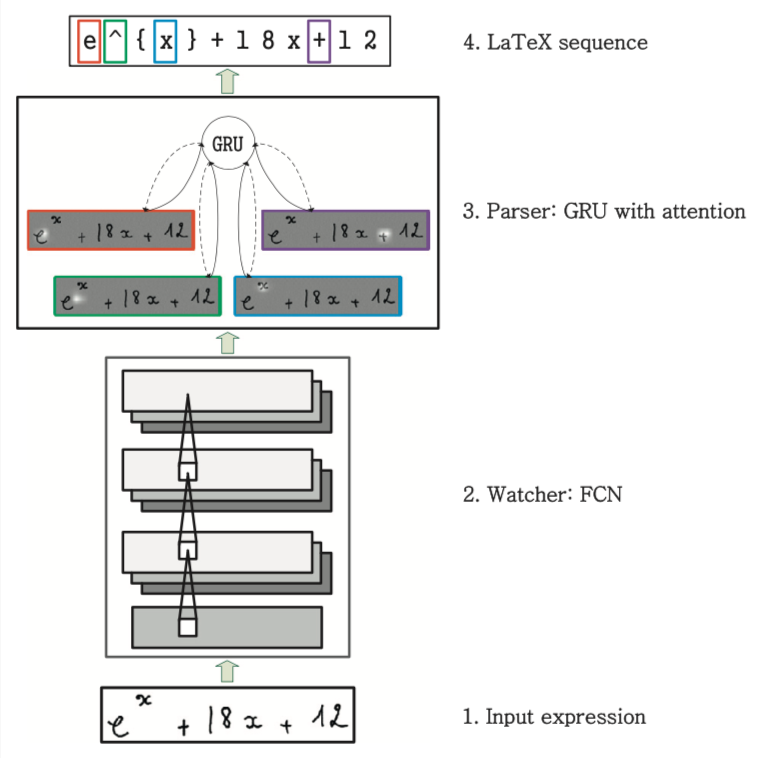
\includegraphics[]{capitulo3/imgs/wap}
	\caption{Diagrama de la arquitectura Watch, Attend, Parse (WAP).}
	\label{fig:wap}
\end{figure}

La red WAP, se compone de dos partes:

\begin{enumerate}
	\item \textbf{Encoder}: El cual es una CNN que permite extraer las características de la imagen y sumarizarlas en un vector de contexto $C$.
	\item  \textbf{Decoder}: El cual es una LSTM que toma el contexto $C$ y junto con sistema de atención retorna como salida la secuencia de símbolos de \LaTeX, un símbolo a la vez.
\end{enumerate}

